\documentclass{standalone}
\usepackage{verbatim}
\usepackage{mathtools}
\usepackage{tikz}
\usetikzlibrary{positioning}
\begin{document}
\pagestyle{empty}
  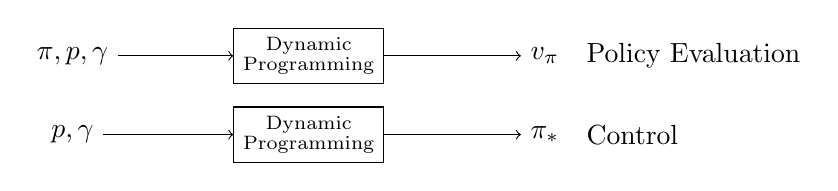
\begin{tikzpicture}
    % Policy eval
    \node (vars) at (0, 0) {$\pi, p, \gamma$};
    \node[draw,rectangle] (dp1) at (3, 0) {$\substack{\textrm{Dynamic} \\         \textrm{Programming}}$};
    \node (vpi)  at (6, 0) {$v_{\pi}$};
    \node[right = 1mm of vpi] {Policy Evaluation};
    \draw[->] (vars) -- (dp1);
    \draw[->] (dp1) -- (vpi);
    % Control
    \node (varsbottom) at (0, -1) {$p, \gamma$};
    \node[draw,rectangle] (dp2) at (3, -1) {$\substack{\textrm{Dynamic} \\         \textrm{Programming}}$};
    \node (pistar)  at (6, -1) {$\pi_*$};
    \node[right = 1mm of pistar] {Control};
    \draw[->] (varsbottom) -- (dp2);
    \draw[->] (dp2) -- (pistar);
  \end{tikzpicture}
\end{document}